\appendix
\chapter{Arbeitsnachweis}

\section{Zeitplan}

\section{Kosten}

\chapter{Programmcode}

\chapter{CAD-Zeichnungen}

<<<<<<< Updated upstream
\chapter{Schaltpläne}

\chapter{Datenblätter}

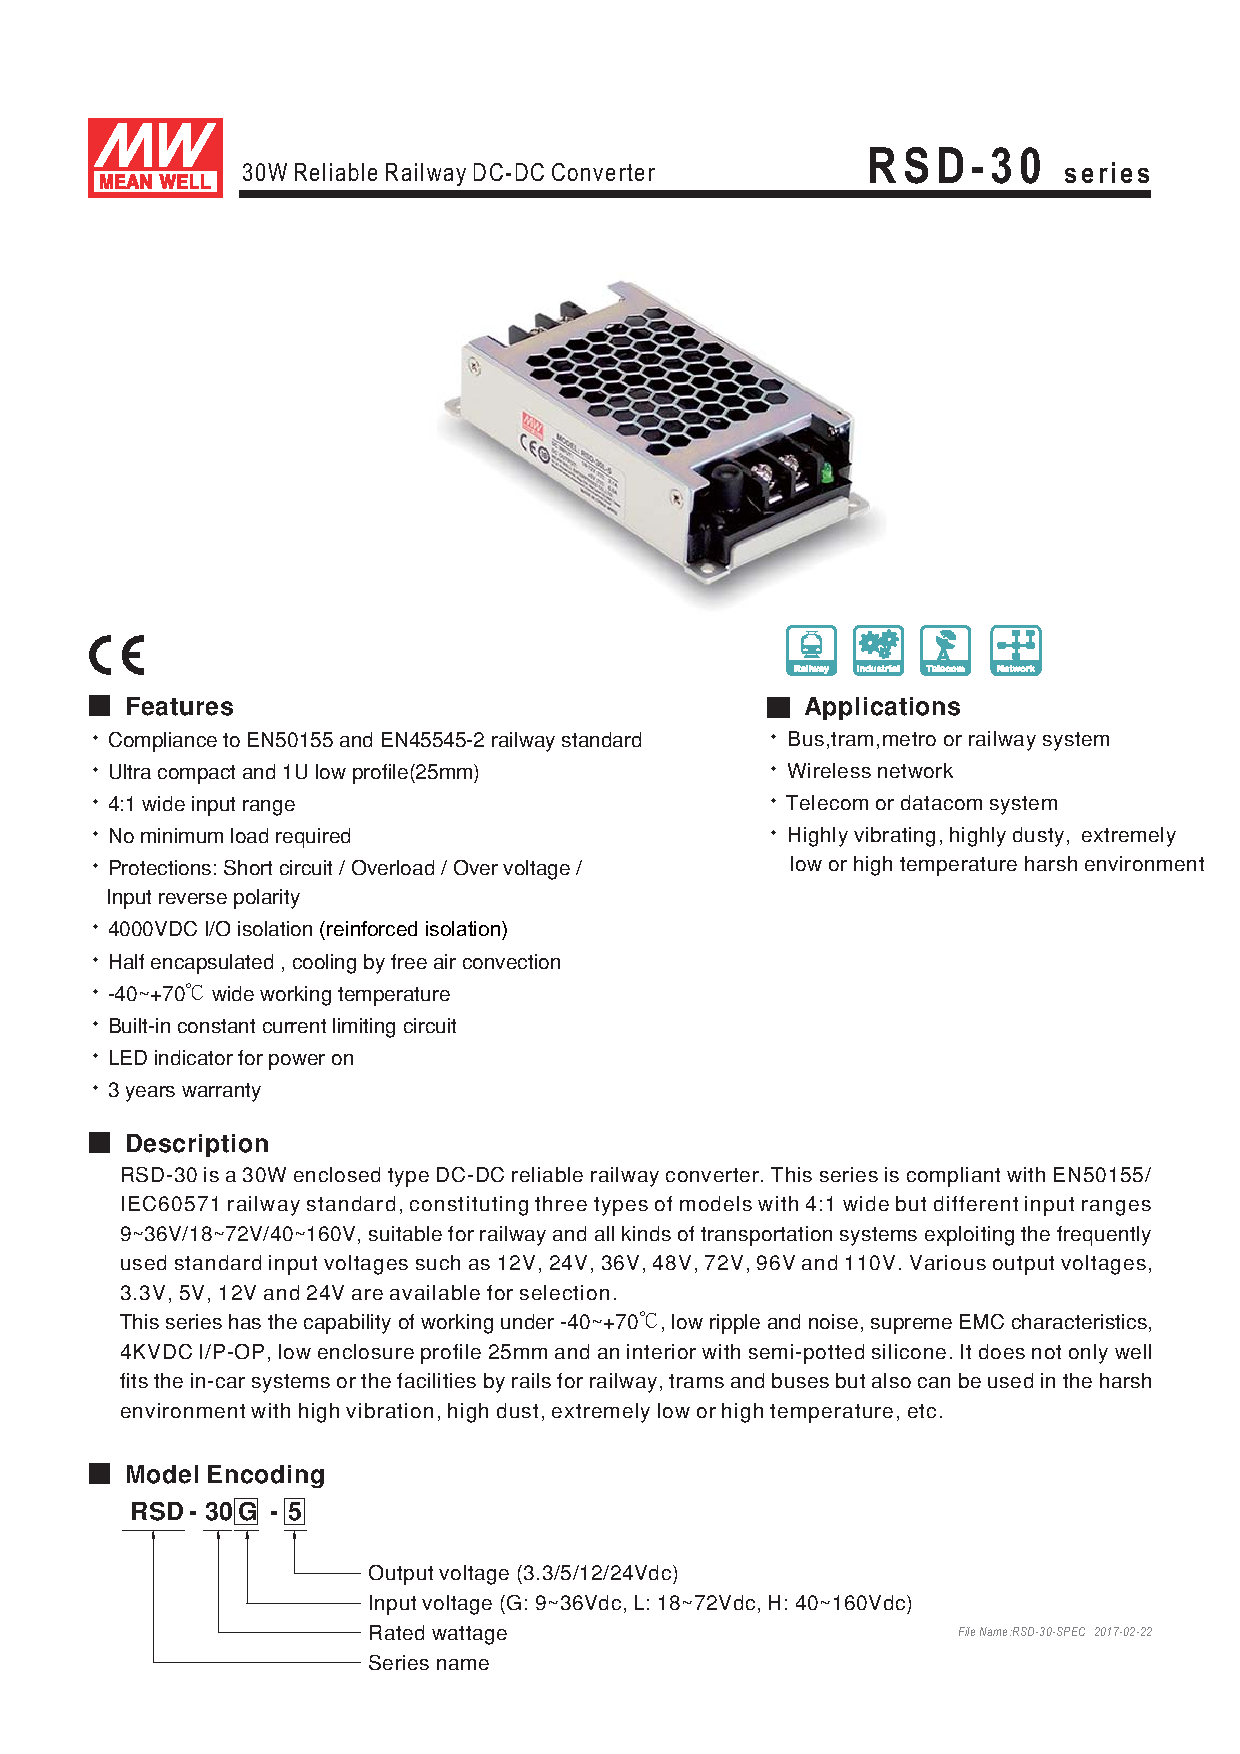
\includepdf[pages=1, pagecommand={\thispagestyle{fancy}}, pagecommand={\subsection{Mean Well RSD-30H-5} \label{app:mw5}}, scale=0.8] {pdf/meanwell5.pdf}
\includepdf[pages=2-, pagecommand={\thispagestyle{fancy}}, scale=0.95] {pdf/meanwell5.pdf}


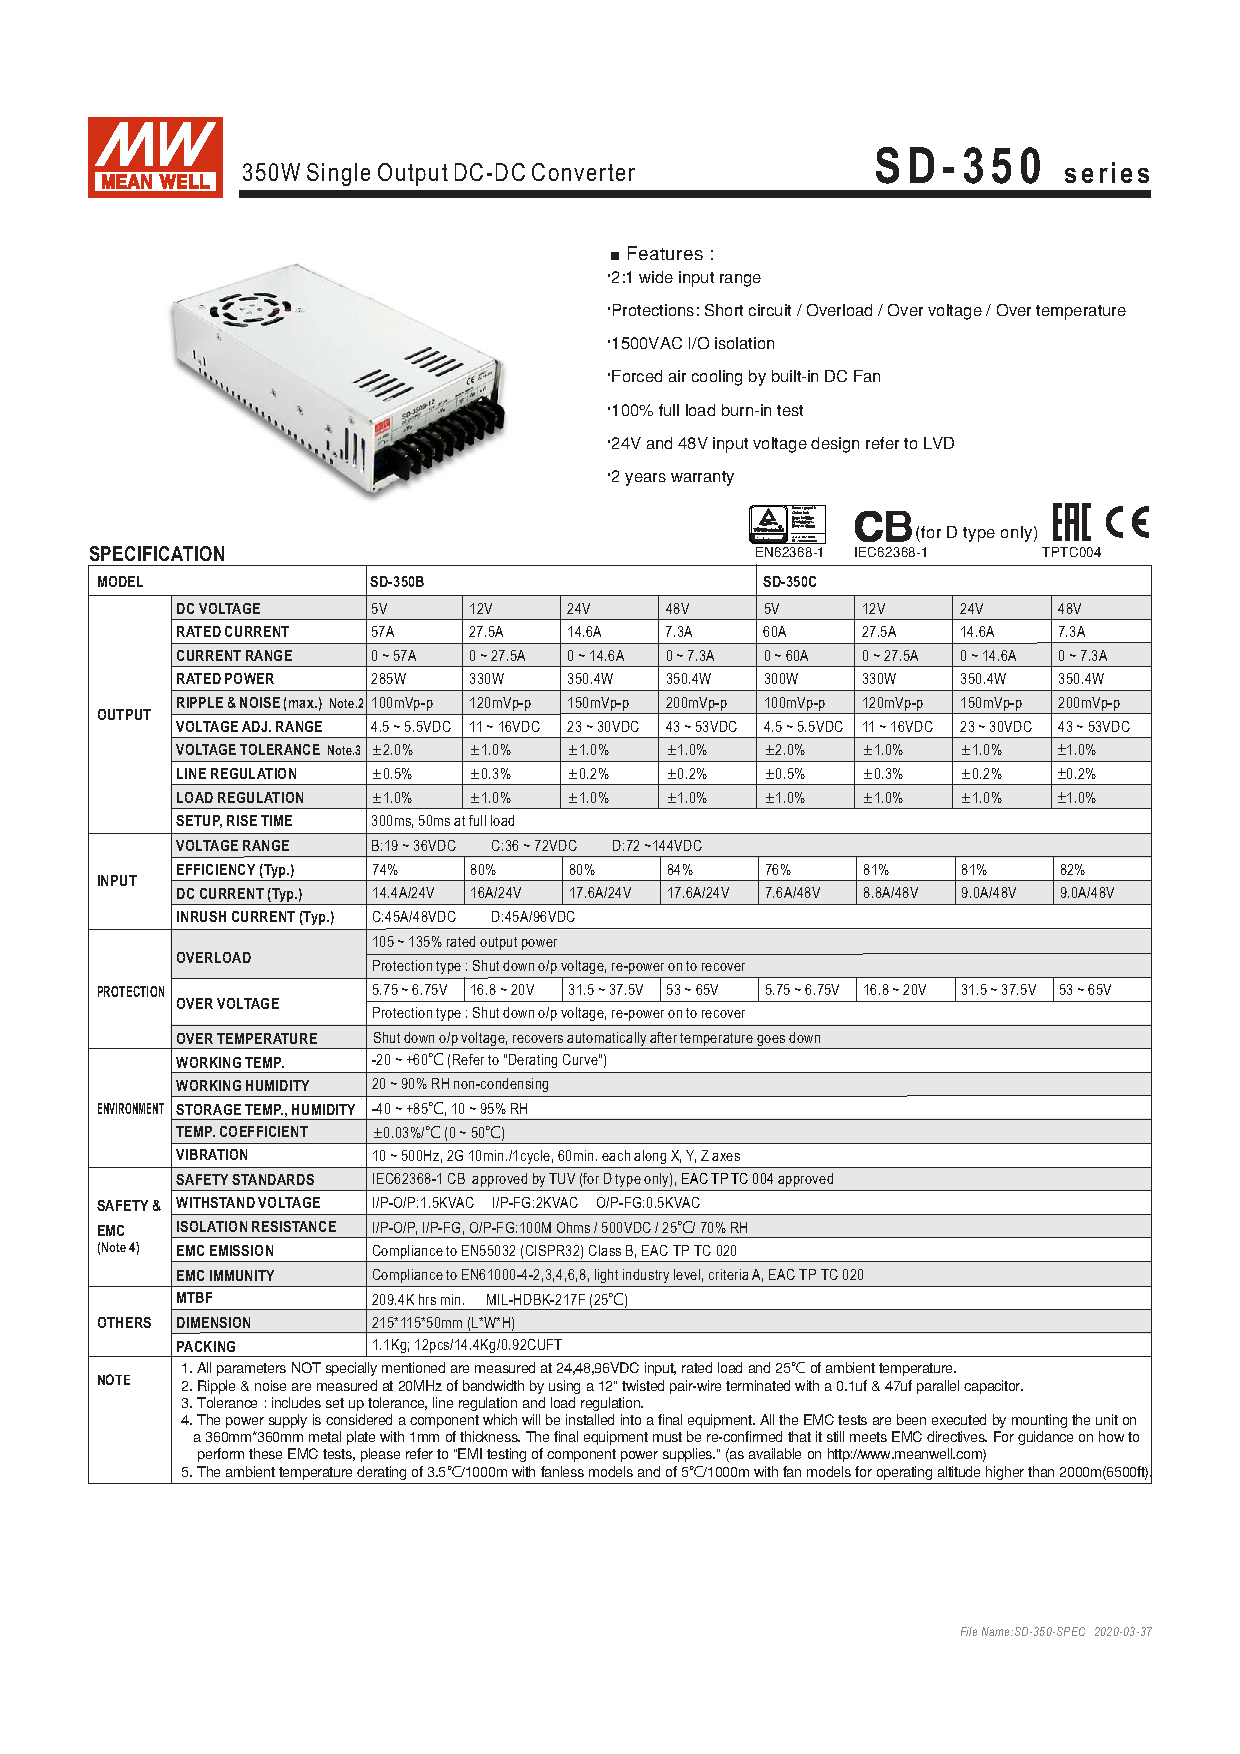
\includepdf[pages=1, pagecommand={\thispagestyle{fancy}}, pagecommand={\subsection{Mean Well SD-350C-12} \label{app:mw12}}, scale=0.8] {pdf/meanwell12.pdf}
\includepdf[pages=2-, pagecommand={\thispagestyle{fancy}}, scale=0.95] {pdf/meanwell12.pdf}


\includepdf[pages=1, pagecommand={\thispagestyle{fancy}}, pagecommand={\subsection{Raspberry Pi 4 Moddel B} \label{app:rasp}}, scale=0.8] {pdf/raspberry.pdf}

\includepdf[pages=2-, pagecommand={\thispagestyle{fancy}}, scale=0.95] {pdf/raspberry.pdf}
=======
\begin{figure} [H]
	\begin{center}
		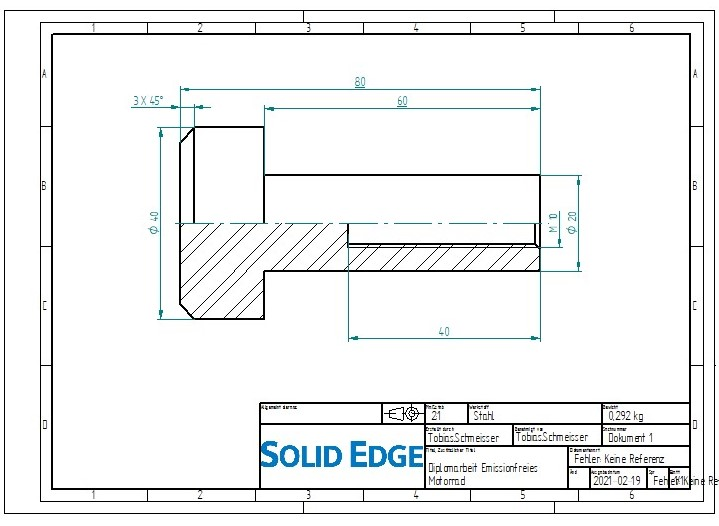
\includegraphics[angle=90] {figures/mechanik/Welle_Rechts_Zeichnung.jpg}
			\caption{Wellenersatz}
			\label{fig:Wellenersatz}
	\end{center}
\end{figure}


\begin{figure} [H]
	\begin{center}
		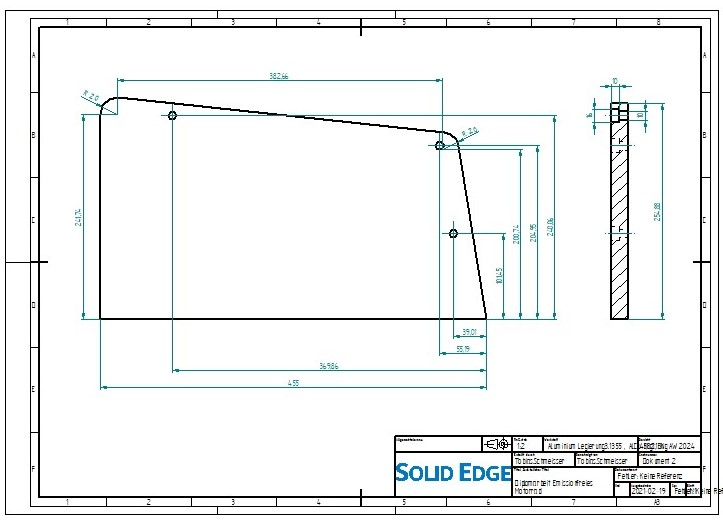
\includegraphics[angle=90]{figures/mechanik/Seitenplatte_Fertigung_Rechts.jpg}
			\caption{Seitenplatte Rechts}
			\label{fig:Seitenplatte Rechts}
	\end{center}
\end{figure}


\begin{figure} [H]
	\begin{center}
		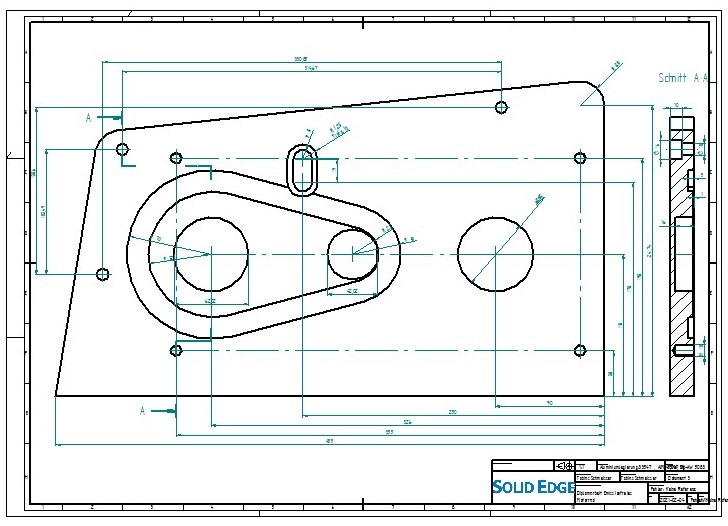
\includegraphics[angle=90]{figures/mechanik/Seitenplatte_Fertigung_Links.jpg}
			\caption{Seitenplatte Links}
			\label{fig:Seitenplatte Links}
	\end{center}
\end{figure}


\begin{figure} [H]
	\begin{center}
		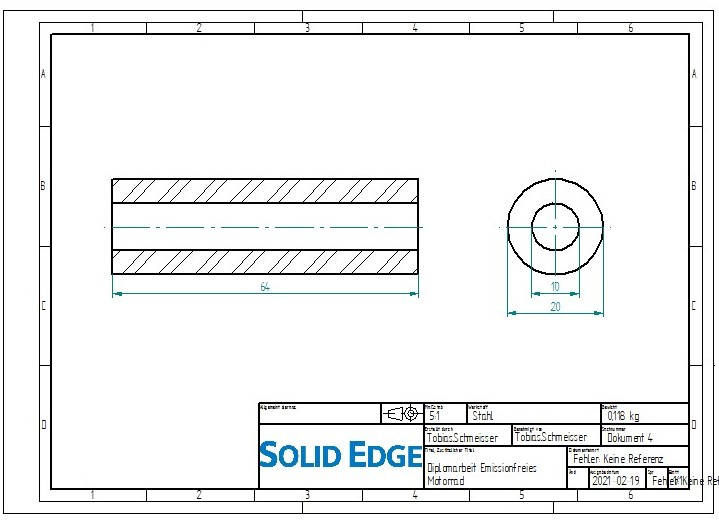
\includegraphics[angle=90]{figures/mechanik/Seitenplatte_Abstandhalter_Zeichnung.jpg}
			\caption{Abstandhalter}
			\label{fig:Abstandhalter}
	\end{center}
\end{figure}


\begin{figure} [H]
	\begin{center}
		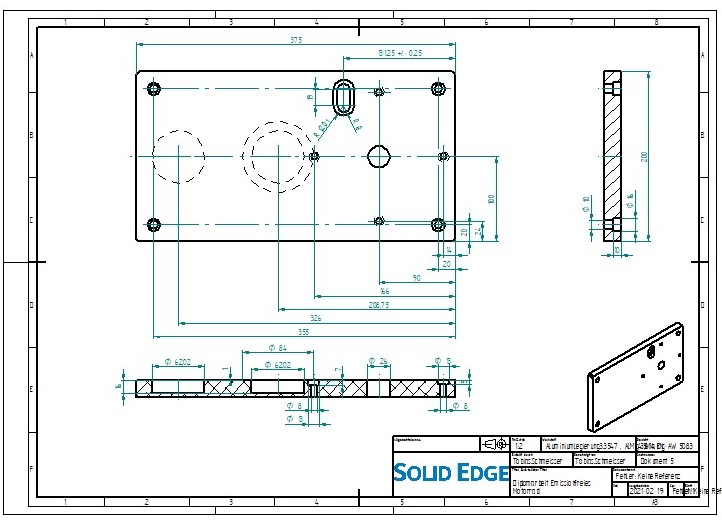
\includegraphics[angle=90]{figures/mechanik/Aufbau_Seitenplatte_Links_Zeichn.jpg}
			\caption{Aufbau/Zusatzplatte}
			\label{fig:Aufbau/Zusatzplatte}
	\end{center}
\end{figure}


\begin{figure} [H]
	\begin{center}
		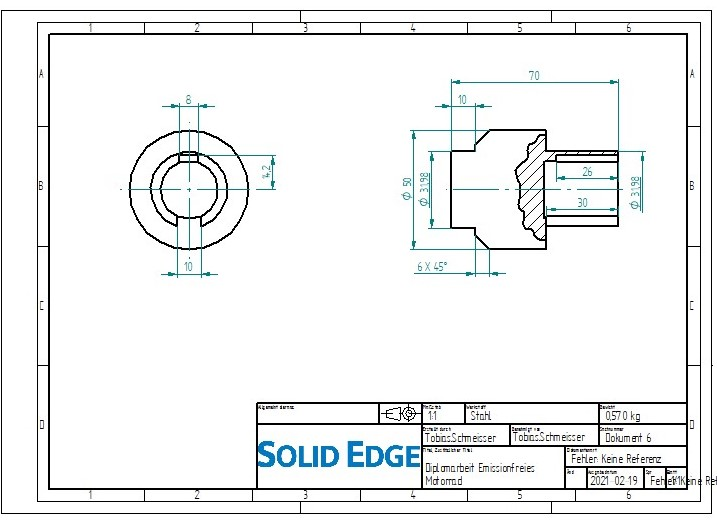
\includegraphics[angle=90]{figures/mechanik/Antriebsachse_Zeichnung.jpg}
			\caption{Achse 1/Antriebsachsen}
			\label{fig:Achse 1/Antriebsachsen}
	\end{center}
\end{figure}


\begin{figure} [H]
	\begin{center}
		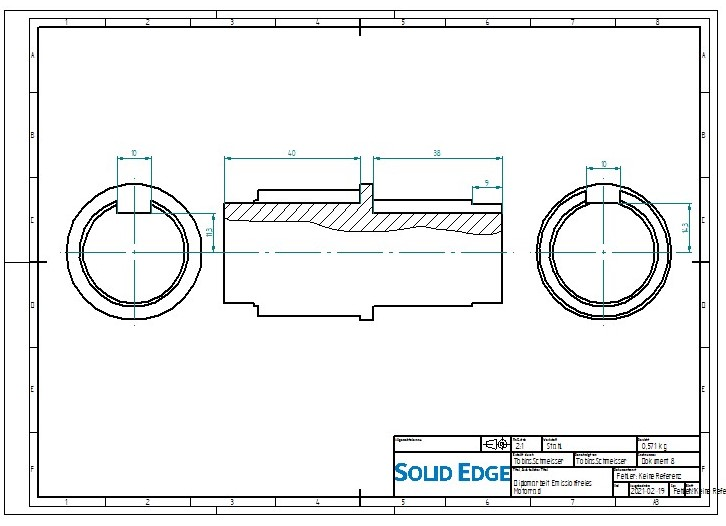
\includegraphics[angle=90]{figures/mechanik/Achse_mit_nuten_Zeichnung.jpg}
			\caption{Achse 3}
			\label{fig:Achse 3}
	\end{center}
\end{figure}


\begin{figure} [H]
	\begin{center}
		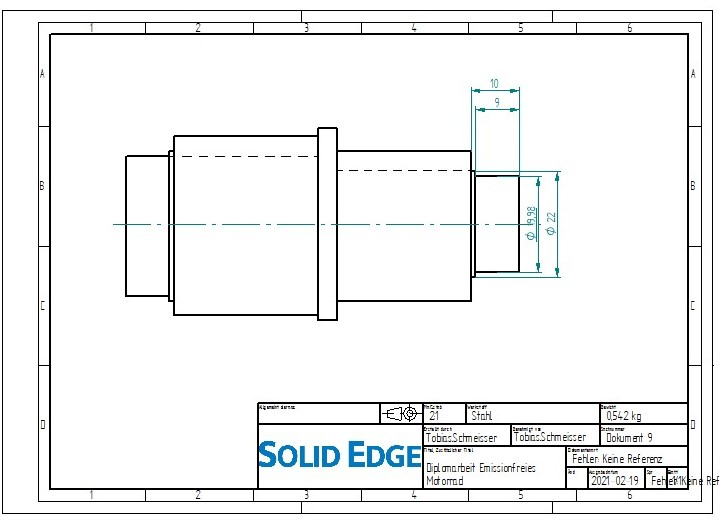
\includegraphics[angle=90]{figures/mechanik/Achse_mit_nuten_20mm_Zeichnung.jpg}
			\caption{Achse 2}
			\label{fig:Achse 2}
	\end{center}
\end{figure}


\begin{figure} [H]
	\begin{center}
		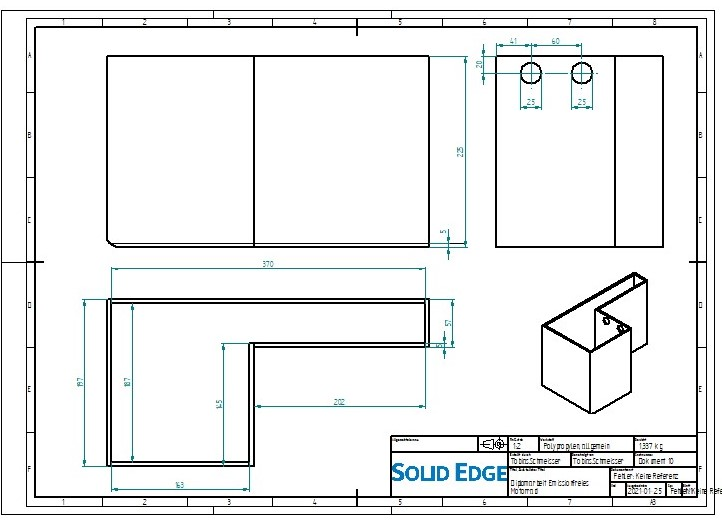
\includegraphics[angle=90]{figures/mechanik/Box_Zeichnung.jpg}
			\caption{Akkubox Motorblock}
			\label{fig:Akkubox Motorblock}
	\end{center}
\end{figure}


\begin{figure} [H]
	\begin{center}
		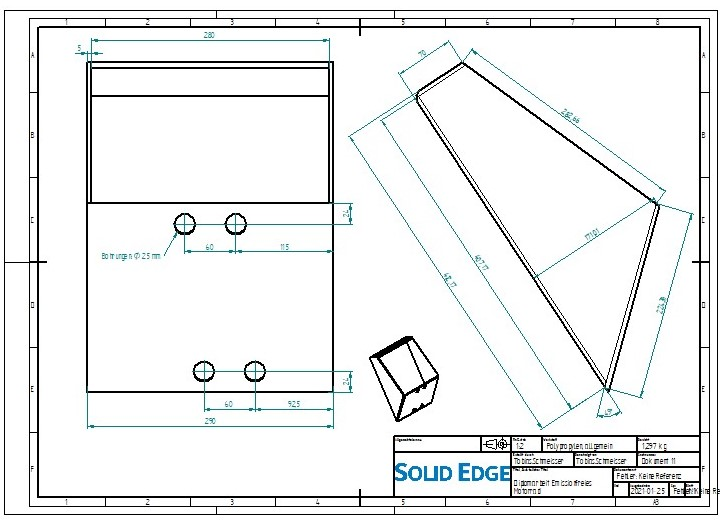
\includegraphics[angle=90]{figures/mechanik/Box_2_Zeichnung.jpg}
			\caption{Akkubox Vorderseite}
			\label{fig:Akkubox Vorderseite}
	\end{center}
\end{figure}


\begin{figure} [H]
	\begin{center}
		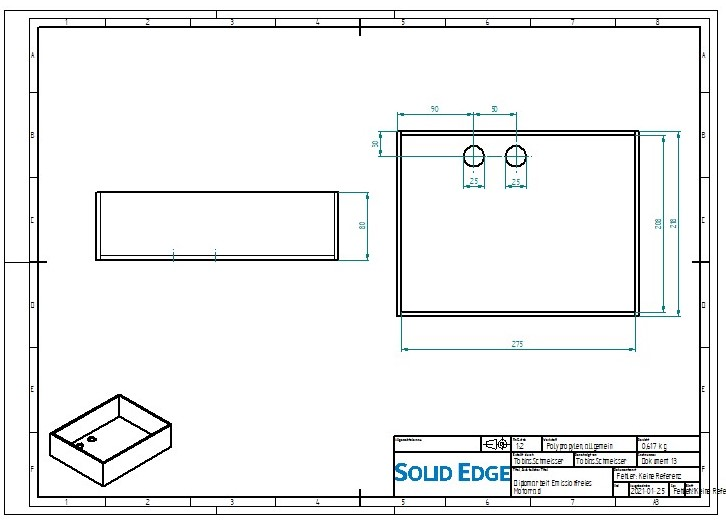
\includegraphics[angle=90]{figures/mechanik/Box_3_Zeichnung.jpg}
			\caption{Akkubox Mitte}
			\label{fig:Akkubox Mitte}
	\end{center}
\end{figure}


\chapter{Solid Edge Simulationen}


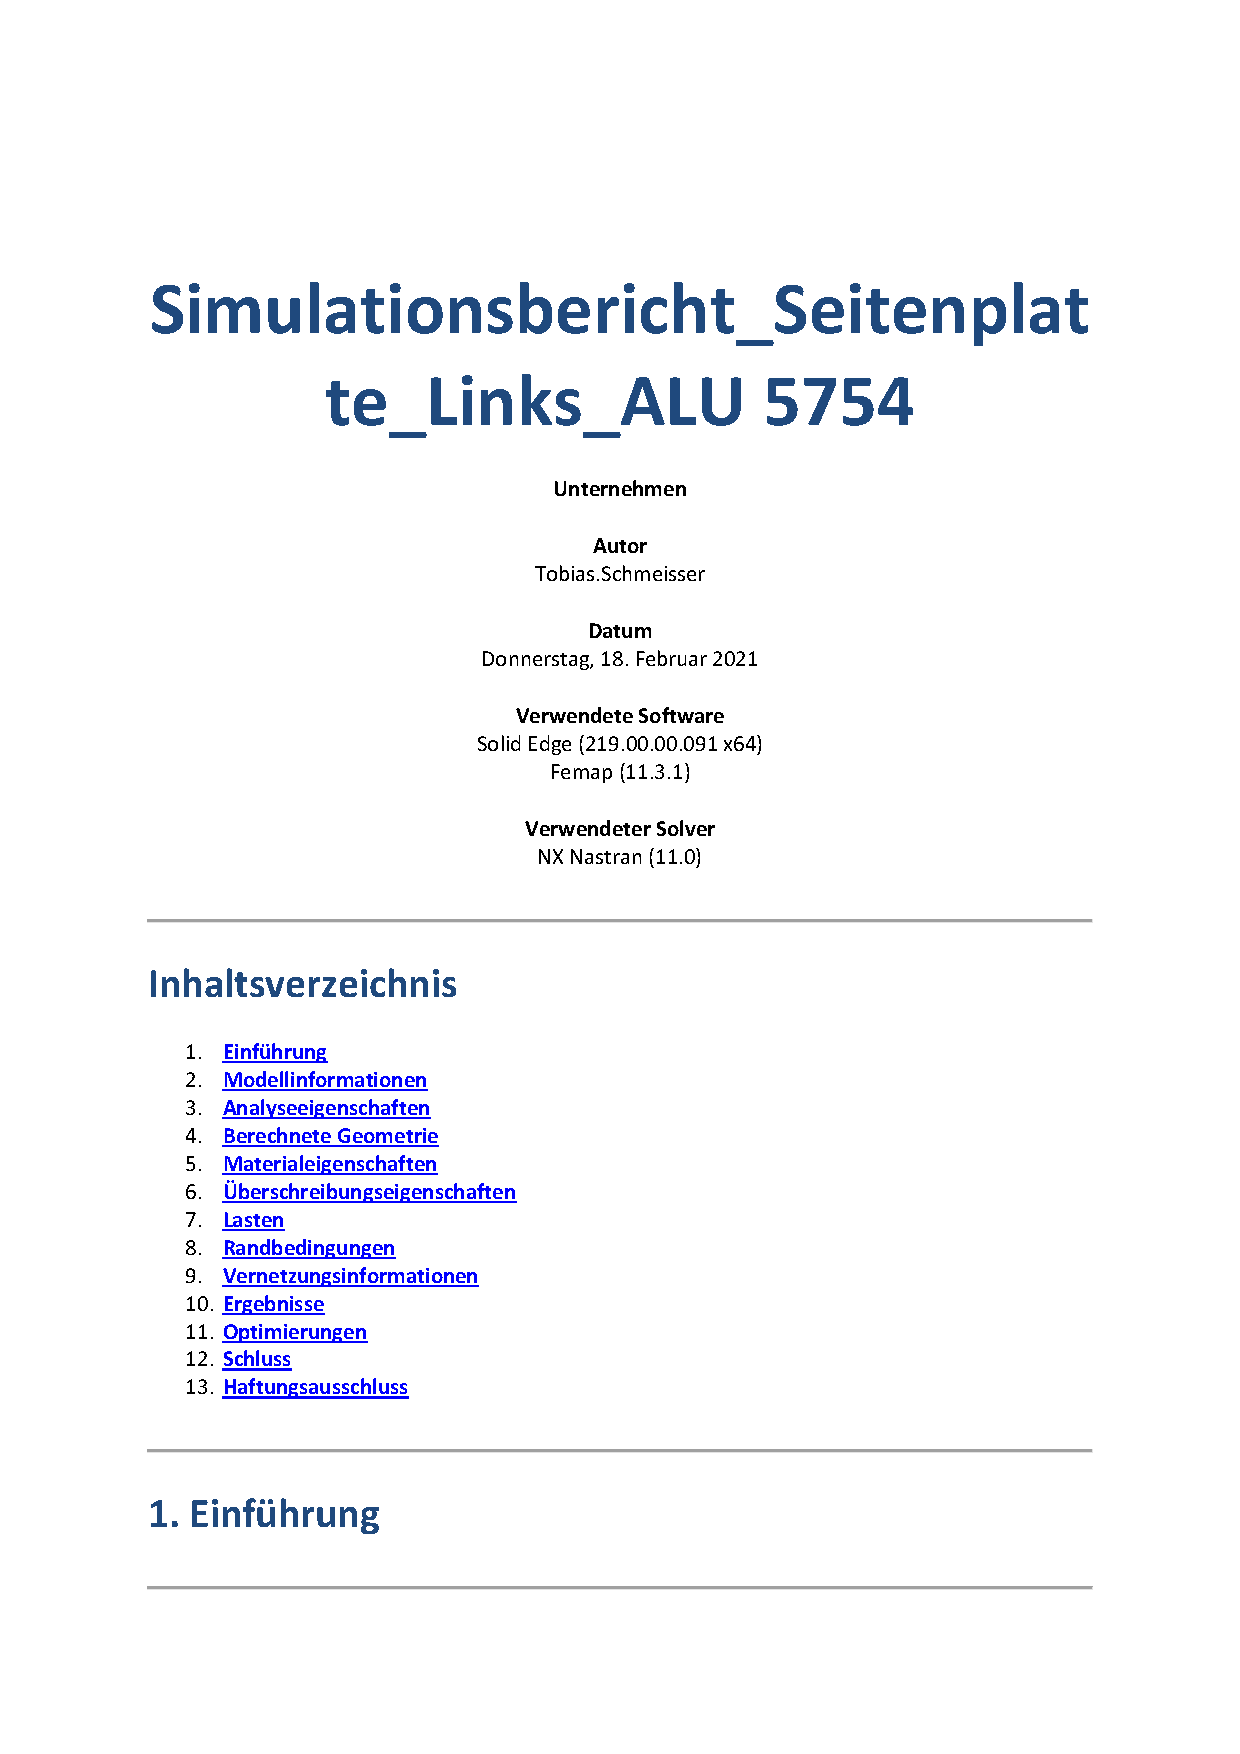
\includepdf [pages=-]{figures/mechanik/Simulationen/Seitenplatte_Links_Statische Berechnung 1_3.pdf}




\includepdf[pages=-]{figures/mechanik/Simulationen/Seitenplatte_Rechts_Statische Berechnung 1_3.pdf}


\chapter{Schaltpläne}
>>>>>>> Stashed changes
